\section{Schieten met het lasergeweer}
\label{app:schieten}
Men kan opmerken uit figuur \ref{fig:UI} dat de schietrichting niet meteen duidelijk uit de gebruikersomgeving wordt. Immers, het vizier wordt niet op hetzelfde punt als het wapen op het scherm afgebeeld. Aangezien het vizier eenvoudiger is om mee te richten dan het wapen, wordt bij het schieten een laserstraal afgevuurd vanuit het wapen naar het punt waar het vizier op gericht staat. Dit is te zien in figuur \ref{fig:COL}. Als het vizier niet op een object gericht staat, dan zal, bij het schieten, de laserstraal uit het wapen afgevuurd worden in de kijkrichting.

\begin{figure}[H]
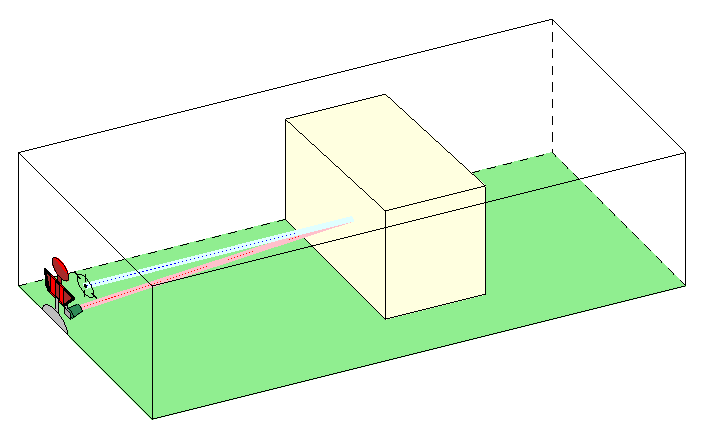
\includegraphics[width=0.9\textwidth]{../Graphics/Collision.eps}
\caption{Een voorbeeld van het schieten van het wapen, de blauwe lijn is niet zichtbaar tijdens het spelen}
\label{fig:COL}
\end{figure}

Een probleem ontstaat wanneer er een object de laserstraal vanaf het wapen naar het punt, waar het vizier op gericht staat, blokkeert. Het object zou dan geraakt moeten worden en niet het punt waar het vizier op gericht staat. Er zijn twee manieren om dit op te lossen, men kan zeggen dat de laser altijd het punt van de vizier raakt. Dit is makkelijker te implementeren, aangezien we maar \'e\'en keer hoeven te bepalen waar een lijn een object raakt. Dit is te zien in figuur \ref{fig:COL2}. Een andere oplossing is dat in dit geval de laser alleen het object, dat in de weg staat, raakt. Dit is natuurlijk realistischer, maar minder makkelijk te implementeren. Dit is te zien in figuur \ref{fig:COL3}. In eerste instantie kiezen wij voor de eerste methode. Echter, indien de tijd ons de mogelijkheid gunt om de tweede oplossing te kunnen implementeren, zullen wij de tweede oplossing implementeren.
\FloatBarrier
\begin{figure}[H]
\begin{subfigure}{0.45\textwidth}
\centering
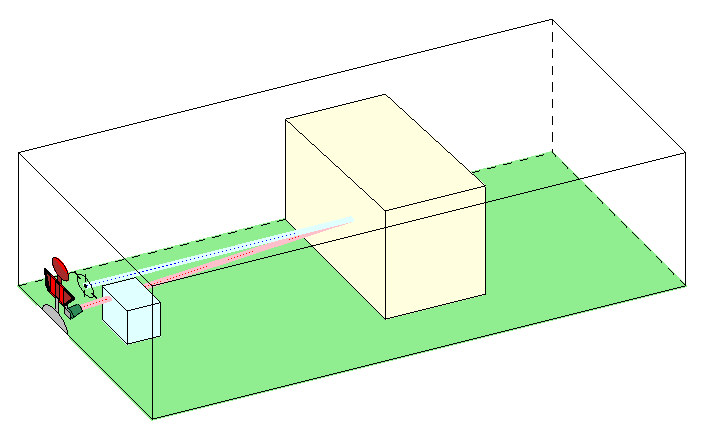
\includegraphics[width=\textwidth]{../Graphics/Collision2.eps}
\caption{De laser komt altijd aan op het punt aangewezen door het vizier}
\label{fig:COL2}
\end{subfigure}
\begin{subfigure}{0.45\textwidth}
\centering
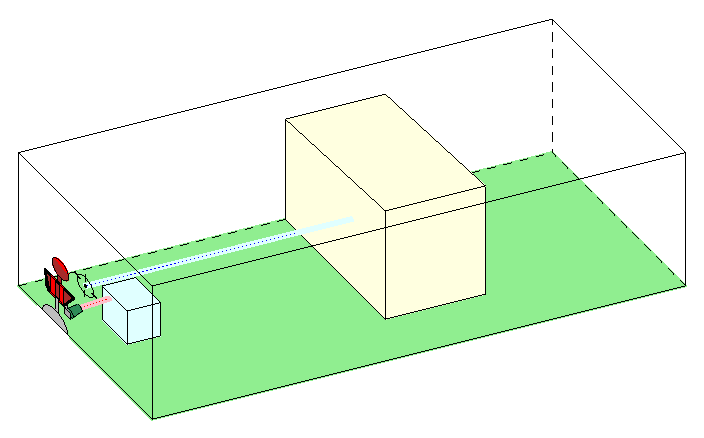
\includegraphics[width=\textwidth]{../Graphics/Collision3.eps}
\caption{De laser stopt zodra hij een ander object raakt}
\label{fig:COL3}
\end{subfigure}
\caption{Oplossingen voor de problemen bij het schieten}
\end{figure}